\section{Tissue segmentation}

% Implement a Gaussian Mixture Model (GMM) to segment the 20 non-segmented MRI brains and optimise your model through an Expectation-Maximisation scheme [15].

\subsection{Expectation-Maximisation}
In order to perform the tissue classification, an Gaussian Mixture Model (GMM) using Expectation-Maximisation (EM) optimisation algorithm has been implemented following \cite{leemput_automated_1999-1}. The initial version that has been developed receives as input the $T_1$-weighted image and the number of classes. The means and variances of the gaussian functions representing each class are initialised randomly, and scaled using the image values:

\begin{equation}
  \mu_k = [\max(y) - \min(y)] R + \min(y)
\end{equation}
and
\begin{equation}
  \sigma^2_k = a R + b [\max(y) - \min(y)]
\end{equation}
where $\mu_k$ is the mean intensity of class $k$, $y$ is the T1 image, $R \sim \mathcal{U}\{0, 1\}$ and $a$ and $b$ are scaling parameters that have been set to 10 and 0.8, respectively.

Once the gaussians parameters have been initialised, the EM loop is run until convergence or until a maximum number of iterations has been reached. The convergence happens when the ratio between the log-likelihood of the current and previous iterations is greater than $1 - \epsilon$, where the convergence threshold $\epsilon$ has been set to $10^{-5}$. The algorithm usually converges around 12 iterations, and the maximum number of iterations has been set to 30. All these parameters are customisable by the user when calling the EM method.

When the EM loop is finished, each voxel is assigned to the class with the highest probability and a label map representing the automatic segmentation is saved. Figure \ref{fig:em-first} shows the results of a segmentation. Dice scores are computed comparing each label with the provided label maps, that are used as ground truth. Since no spatial information is used, the algorithm has assigned voxels outside the brain to be brain tissue, and some voxels are isolated within a different class, which is is not plausible anatomically. Adding TPMs as priors and using Markov random field (MRF) smoothing is necessary to produce a more realistic output.

\begin{figure}
  \centering
  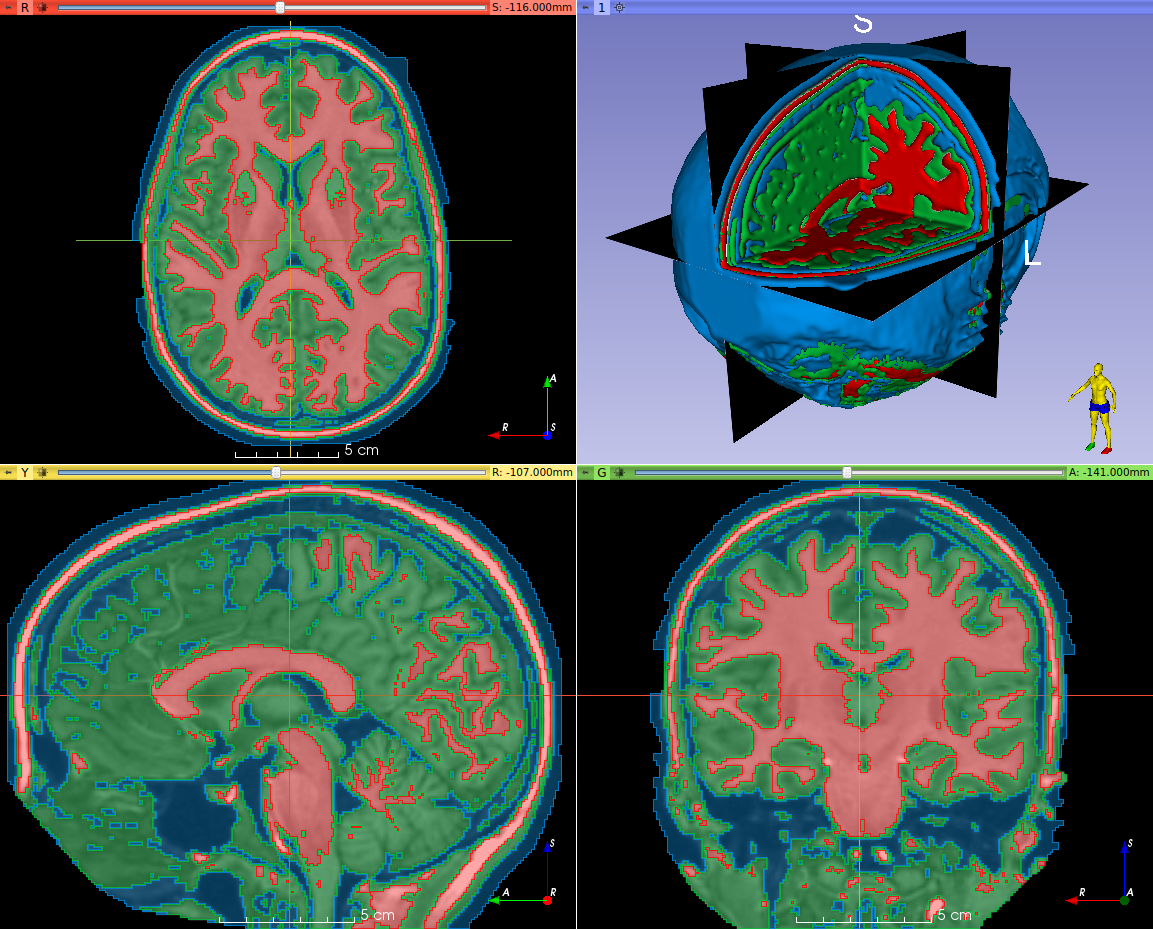
\includegraphics[width=\textwidth]{figures/em_first}
  \caption{Results of an automatic EM segmentation. Approximate classes are: blue - CSF; green - GM; green - WM.}
  \label{fig:em-first}
\end{figure}

The uncertainty of the algorithm assigning a voxel $i$ to a class can be measured as $u_i = 1 - \sigma_i$. Figure \ref{fig:experiment-a} shows another representation of the segmentation of this experiment (named A), including the uncertainty image. The most certain zones are the background and the inner parts of the WM, while the most uncertain ones are the interfaces between different tissues.


\begin{figure}
  \centering
  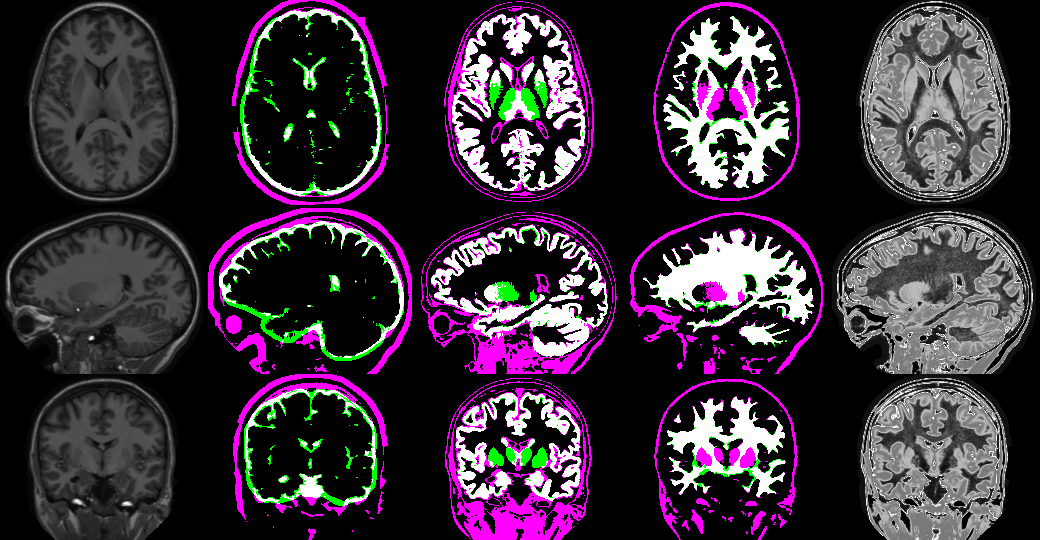
\includegraphics[width=0.7\textwidth]{figures/experiment_a}
  \caption{Results of experiment A.}
  \label{fig:experiment-a}
\end{figure}




% Use image registration to propagate the previously generated tissue probability maps into the space of the non-segmented brain MRIs. This can be achieved by registering the groupwise mean template to the non- segmented brain and then applying the obtained transformation to the probability maps.

\subsection{Initialisation using tissue priors}
In order to use the previously generated TPMs as priors for the GMM, they must be propagated to the subject's space. For that, the template image is non-linearly registered to the subject's $T_1$-weighted MRI and the resulting transform is applied to the TPMs.

% TODO: explain choice of reg_f3d bending energy
% Since the TPMs and the template have been built with linear registrations only, the same logic must be applied while propagating them. This means that the free-form registration must be flexible enough to adapt to the subject's anatomy while producing a smooth resampled TPM that ensures a certain generalisability.

% TODO: show displacement field and jacobian

% Use then the propagated probability maps as a priori information in your GMM [10]. If you did not complete the previous section, you may use the provided prior files.

Once the TPMs are projected into the subject's space, they can be used as priors within the bayesian framework implemented in the EM algorithm. Adding this spatial a priori leads to better qualitative and cuantitative results, as shown in Figure \ref{fig:em-priors}.

\begin{figure}
  \centering
  \includegraphics[width=0.7\textwidth]{figures/em_priors}
  \caption{Results of an automatic EM segmentation using TPMs as priors. The different classes are: blue - CSF; green - GM; green - WM. The Dice scores compared to the provided segmentation are: 0.80 for CSF, 0.90 for GM and 0.92 for GM.}
  \label{fig:em-priors}
\end{figure}

% TODO: show segmentation with priors. And uncertainty?


\subsection{Regularisation with Markov random fields}

% Embed a Markov random field into your segmentation framework to introduce a spatial smoothness term in the label estimation process [10].

Noise or bright voxels outside the brain can make the intensity of a voxel different to its neighbors intensities, which may lead to isolated voxels if the a priori probabilities for different classes are similar. Embedding a Markov random field (MRF) into the segmentation helps smoothing the labels, potentially improving the anatomical plausibility of the segmentation. More specifically, a sixth-order Gibbs Random Field has been implemented. The probabilities array is multiplied by $e^{- \beta U_{MRF}(.)}$, where $U_{MRF}$ is the energy function of the MRF and $\beta$ is a weighting parameter used to control the effect of the MRF on the segmentation. Figure \ref{fig:em-mrf} shows the results of a segmentations that include MRF smoothing, for different values of $\beta$. The results show that the labels smoothing increases with $\beta$.

% TODO: show segmentations with MRF. Explain better using literature


\subsection{Bias field correction}

% MRI acquisition usually suffers from intensity non-uniformity (INU), improve the robustness of your GMM framework to INU by adding a bias field correction component to the probabilistic model [5].

Since MRI acquisition usually suffers from intensity non-uniformity (INU) due to inhomogeneities in the static magnetic field of the MR scanner, a bias field correction component has been also embedded into the segmentation framework. The bias field is modelled using three-dimensional polynomials whose coefficients are computed using a weighted least-squares fit, as in \cite{leemput_automated_1999}. The implemented algorithm can use polynomial orders from 0 to 3.

The computed bias field can saved, as shown in Figure \ref{fig:bias-field}. Most of the exctracted bias fields from the images look similar: bright in the head and darker outside it. This might be due to two reasons:
\begin{enumerate}
  \item The images used for this project have already been preprocessed to remove some of the intrinsic bias field artefact
  \item The algorithm tries to remove bias from the voxels classified as background, which is not useful in this case. A possible extension of the classification algorithm would be using only the foreground voxels for the bias field correction step.
\end{enumerate}
Therefore, small changes in the quality of the segmentation are expected when using the INU correction step.

\begin{figure}
  \centering
  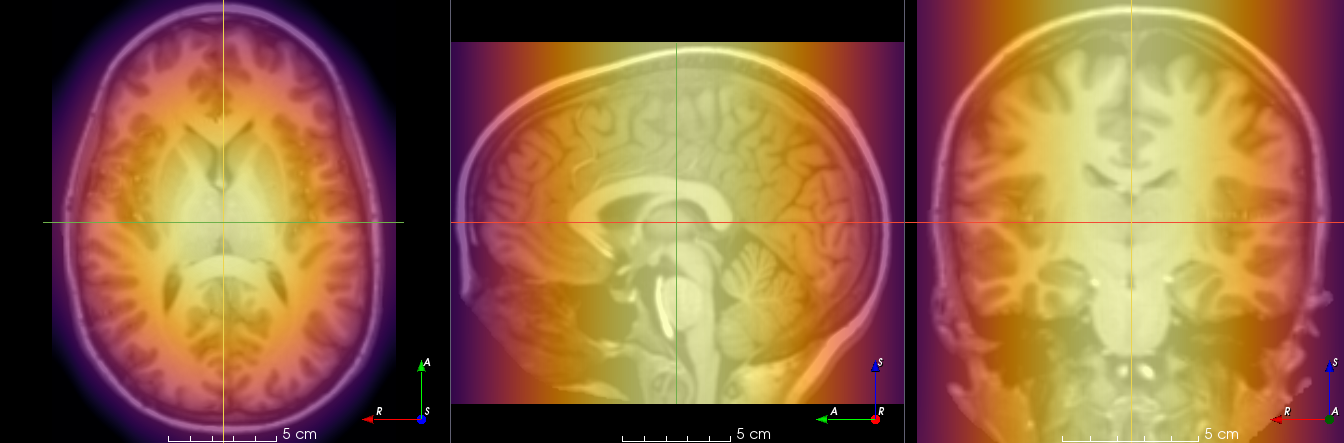
\includegraphics[width=\textwidth]{figures/bias_field}
  \caption{Estimated bias field superimposed on the $T_1$-weighted image. Higher intensity represents larger bias.}
  \label{fig:params-optimisation}
\end{figure}


\subsection{Similarity measure}

% TODO: explain Dice, weighted?




\subsection{Parameters optimisation}

% Use one already segmented images to optimise your implementation parameters (e.g. INU complexity, MRF beta term) [10].

A regular parameter grid has been generated in order to sample the parameter space looking for the best Dice scores, using the first segmented subject. The polinomial orders were 0, 1, 2 and 3 and 8 values of $\beta$ in a logarithmic space from 0.01 to 2 have been sampled. Figure \ref{fig:params-optimisation} shows the results of this parameters search. Interpolating the Dice scores using bicubic interpolation shows that a good choice for the polynomials order is 2 or 3, while $\beta$ should be lower than 1 for good scores. Following segmentation experiments have been performed with polynomial order $n = 2$ and MRF weight $\beta = 0.2$.



\begin{figure}
  \centering
  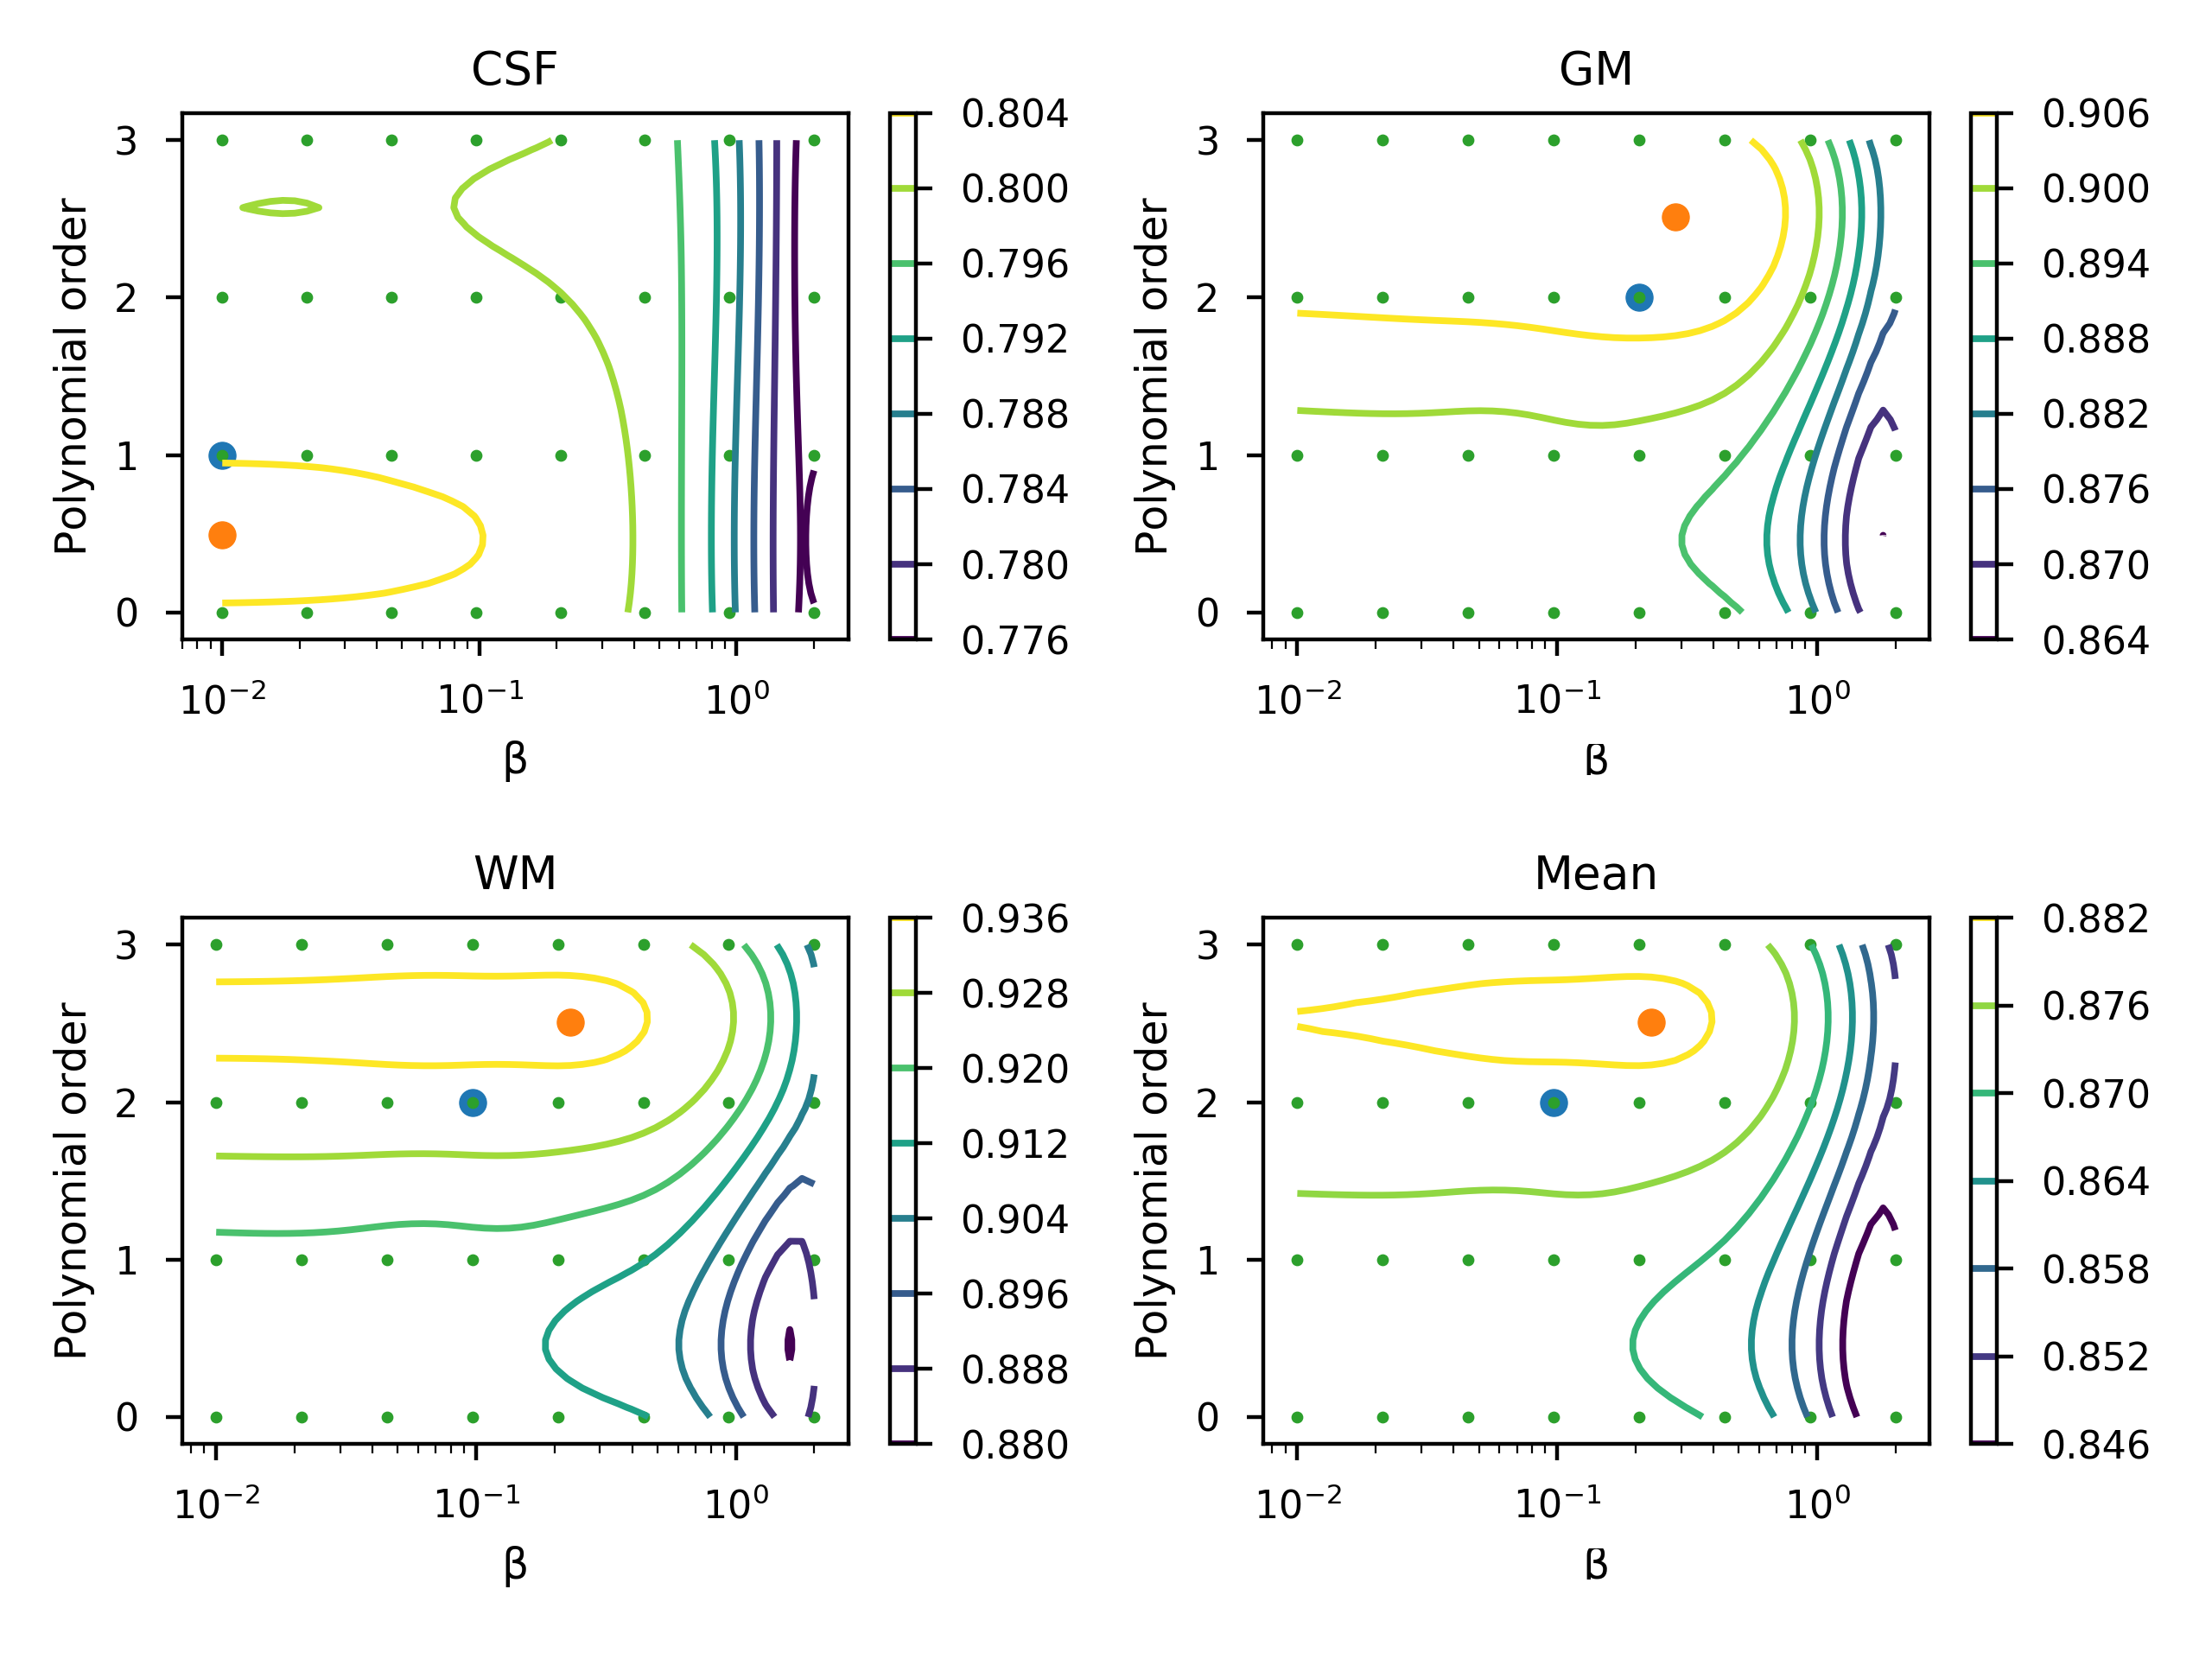
\includegraphics[width=\textwidth]{figures/parameters_dices}
  \caption{Contour plots representing Dice scores for the different parameters. The contours are isolines of the sampled scores interpolated using bicubic interpolation. Green dots represented sampled points; blue dots are the highest sampled Dice score; orange dots are the highest interpolated Dice score.}
  \label{fig:params-optimisation}
\end{figure}


% By choosing these parameters, bias can be introduced in the optimisation. Describe one potential bias and propose a solution to avoid it [5]?

Optimising the segmentation parameters using only data from one subject leads to an overfit towards this subject, as shown in Figure \ref{fig:dices-bars}. If all the subjects were used for the parameters optimisation, the mean Dice score for the whole group would probably be higher.

\begin{figure}
  \centering
  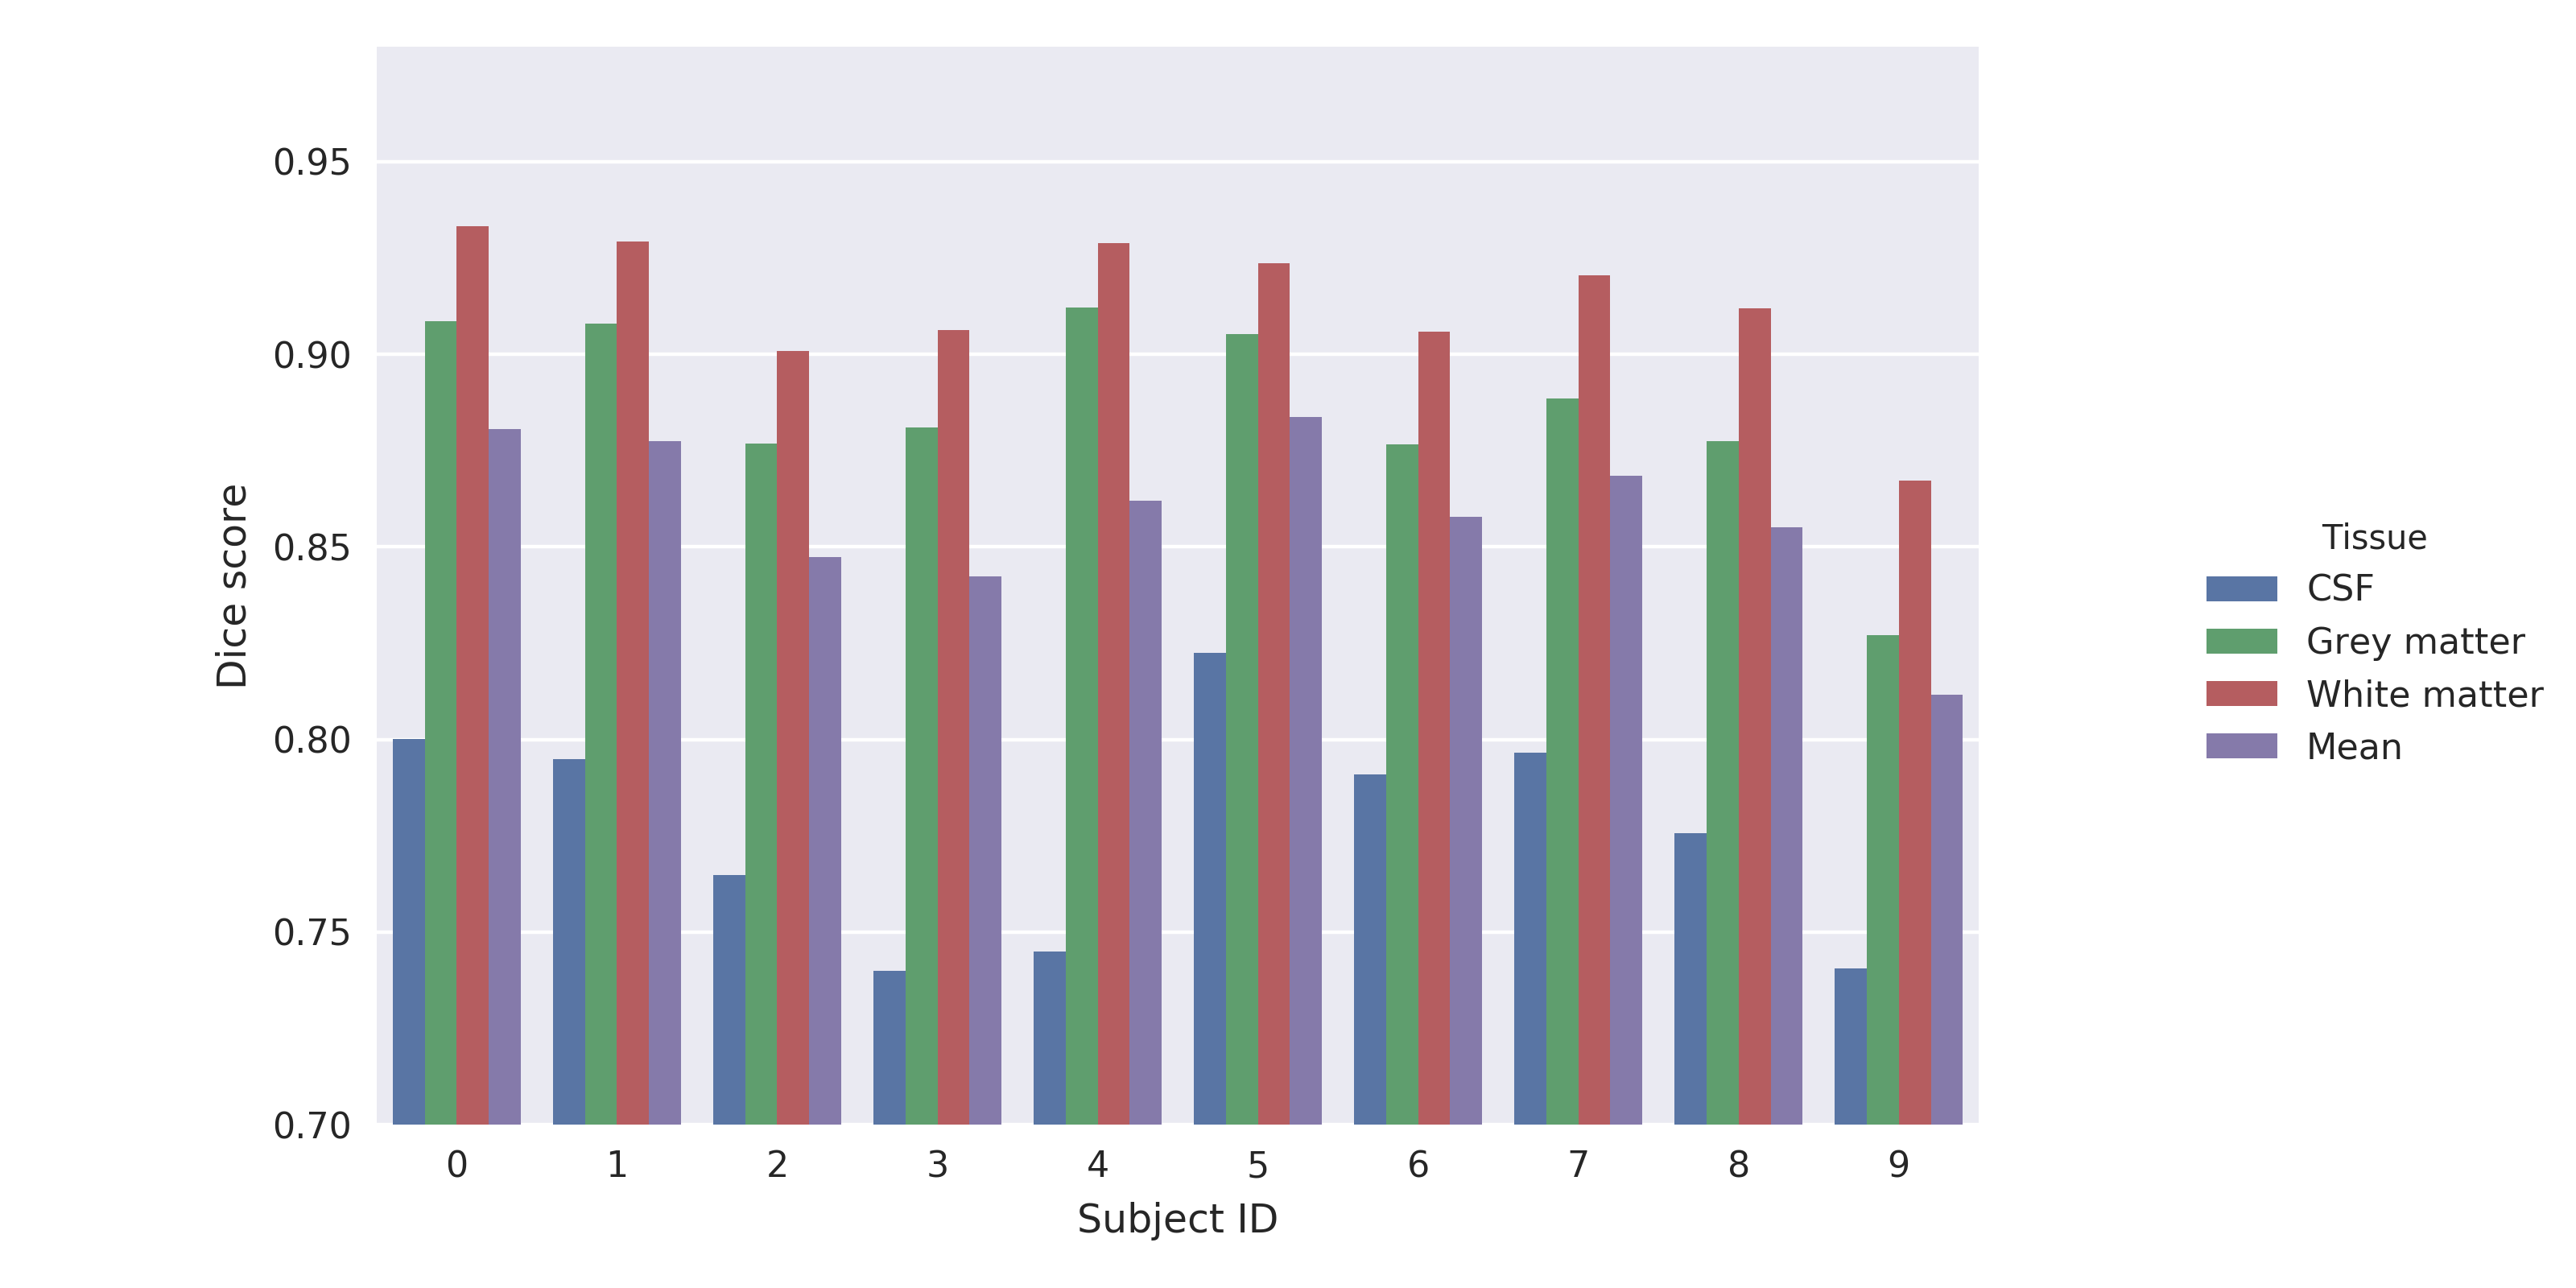
\includegraphics[width=\textwidth]{figures/dices_bars}
  \caption{Dice scores for all segmented subjects. The selected parameters seem to work best for subject 0, the one used for the optimisation. These parameters work well with subject 5 as well. Optimising the parameters using all subjects would probably lead to better results.}
  \label{fig:dices-bars}
\end{figure}
